\section{Task3 --- Encryption Mode --- ECB vs. CBC}
%

\begin{figure}
    \centering
    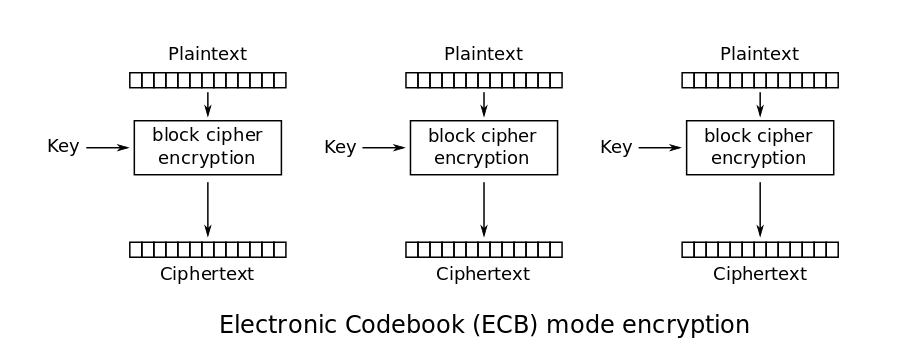
\includegraphics[height=\textheight,width=\textwidth,keepaspectratio]
    {figures/ECB_encryption.png}
    \caption{Electronic Codebook (ECB) mode encryption.}\label{fig:ecb_mode}
\end{figure}

\begin{figure}
    \centering
    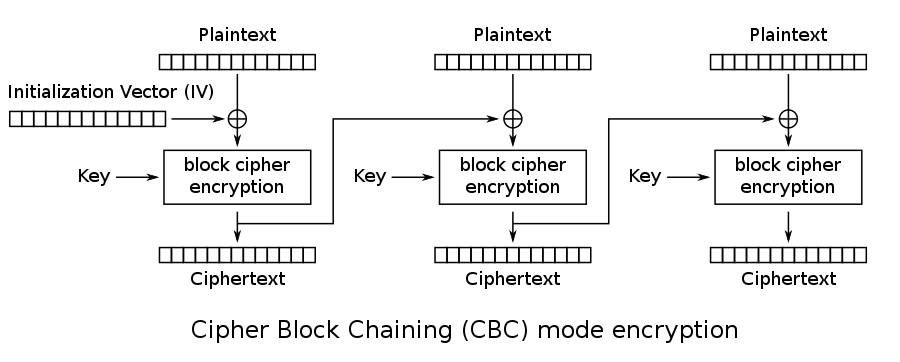
\includegraphics[height=\textheight,width=\textwidth,keepaspectratio]
    {figures/CBC_encryption.png}
    \caption{Cipher Block Chaining (CBC) mode encryption.}\label{fig:cbc_mode}
\end{figure}

In the electronic codebook (ECB) mode, the plaintext is splitted into
blocks which are encrypted separately, as shown in \autoref{fig:ecb_mode}.
The drawback of this mode is a lack of diffusion~\cite{cipher_mode_wiki}.
Identical plaintext blocks are encrypted into identical ciphertext blocks,
exposing the data pattern easily~\cite{ecb_cbc_example}. Two examples below
illustrate this disadvantage. In more detail, while encrypting a bitmap
image, ECB mode encrypts identically-colored original pixels to a uniform
pattern. Hence, the overall pattern of the image can be detected~\cite{cipher_mode_wiki}.
Note that only the pattern of a image which contains large uniform areas
can be discerned easily. Since if a image contains pixels with variant 
color, its encrypted version will look noisy with pseudo-randomly colored
pixels.

In the cipher block chaining (CBC) mode, each plaintext block is XORed with
the previous ciphertext block before being encrypted~\cite{cipher_mode_wiki},
as shown in \autoref{fig:cbc_mode}.
In addition, the first plaintext block is XORed with the initial vector (IV)
before being encrypted. Thus, each block of ciphertext depends on all
previous ciphertext blocks~\cite{cipher_mode_wiki}. This relationship prevents
identical plaintext blocks from producing identical ciphertext blocks~\cite{ecb_cbc_example}.

In the next two subsections, we will observe examples in which bitmap images are
encrypted with both cipher modes.

\subsection{Using picture {\fontfamily{qcr}\selectfont pic\_original.bmp}}
%
\begin{lstlisting}[language=Bash, caption=Commands generating
    {\fontfamily{qcr}\selectfont pic\_cbc.bmp}, label={lst:pic_cbc}]
$ openssl enc -e -des-cbc -salt -pbkdf2 -kfile password.txt \
    -in pic_original.bmp -out pic_original.bmp.cbc # encrypt the original picture
$ head -c 54 pic_original.bmp > header # create a file containing header of a bitmap image
$ tail -c +55 pic_original.bmp.cbc > cbc_body # create a file containing body of an encrypted image

# combine the original header and the encrypted body to
# create a complete encrypted bitmap image
$ cat header cbc_body > pic_cbc.bmp
\end{lstlisting}

Given an original image (\autoref{fig:original_pic}), we can obtain its
overall pattern though it was encrypted with ECB mode, shown in \autoref{fig:ecb_pic}.
Since the original image contains three large uniform-color areas
, including an ellipse (red), a rectangular (green), and a background (white)
, the patterns of these
3 areas are splitted clearly. The reason behind is that uniform areas of
red (green, or white) pixels are encrypted into colored uniform areas, so
we still see these shapes but with another color.

On the other hand, by looking at the output of CBC mode (\autoref{fig:cbc_pic}), we cannot
detect the pattern of the original image as the encrypted version now looks
very noisy.

\begin{lstlisting}[language=Bash, caption=Commands generating
    {\fontfamily{qcr}\selectfont pic\_ecb.bmp}, label={lst:pic_ecb}]
$ openssl enc -e -des-ecb -salt -pbkdf2 -kfile password.txt \
    -in pic_original.bmp -out pic_original.bmp.ecb # encrypt the original picture
$ head -c 54 pic_original.bmp > header
$ tail -c +55 pic_original.bmp.ecb > ecb_body
$ cat header ecb_body > pic_ecb.bmp
\end{lstlisting}

\begin{figure}
    \centering
    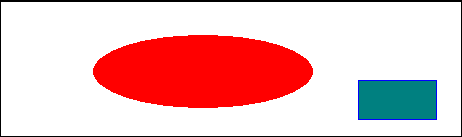
\includegraphics[height=\textheight,width=\textwidth,keepaspectratio]
    {figures/pic_original.png}
    \caption{The original picture.}\label{fig:original_pic}
\end{figure}

\begin{figure}
    \centering
    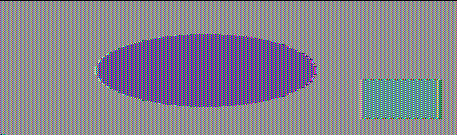
\includegraphics[height=\textheight,width=\textwidth,keepaspectratio]
    {figures/pic_ecb.png}
    \caption{The ECB-mode encrypted picture.}\label{fig:ecb_pic}
\end{figure}

\begin{figure}
    \centering
    
\includegraphics[height=\textheight,width=\textwidth,keepaspectratio]
    {figures/pic_cbc.png}
    \caption{The CBC-mode encrypted picture.}\label{fig:cbc_pic}
\end{figure}

\subsection{Using picture {\fontfamily{qcr}\selectfont snail.bmp}}
%
\begin{lstlisting}[language=Bash, caption=Commands generating
    {\fontfamily{qcr}\selectfont snail\_cbc.bmp}, label={
        lst:snail_cbc
    }]
$ openssl enc -e -des-cbc -salt -pbkdf2 -kfile password.txt \
    -in snail.bmp -out snail.bmp.cbc # encrypt the original picture
$ head -c 54 snail.bmp > snail_header
$ tail -c +55 snail.bmp.cbc > snail_cbc_body
$ cat snail_header snail_cbc_body > snail_cbc.bmp
\end{lstlisting}

Given an original image (\autoref{fig:snail}), we can obtain its
overall pattern though it was encrypted with ECB mode, shown in
\autoref{fig:snail_ecb}.
Since the original image contains two large uniform-color areas
, including the snail (yellow) and the background (white), the patterns of these
2 areas are splitted clearly. The reason behind is that uniform areas of
yellow (or white) pixels are encrypted into colored uniform areas, so
we still see these shapes but with another color. In this case, the snail
itself produced a noisy encrypted pattern as color of the snail is variant.

On the other hand, by looking at the output of CBC mode
(\autoref{fig:snail_cbc}),
we cannot detect the pattern of the original image as the encrypted
version now looks very noisy.

\begin{lstlisting}[language=Bash, caption=Commands generating
    {\fontfamily{qcr}\selectfont snail\_ecb.bmp}, label={
        lst:snail_ecb
    }]
$ openssl enc -e -des-ecb -salt -pbkdf2 -kfile password.txt \
    -in snail.bmp -out snail.bmp.ecb # encrypt the original picture
$ head -c 54 snail.bmp > snail_header
$ tail -c +55 snail.bmp.ecb > snail_ecb_body
$ cat snail_header snail_ecb_body > snail_ecb.bmp
\end{lstlisting}

\begin{figure}
    \centering
    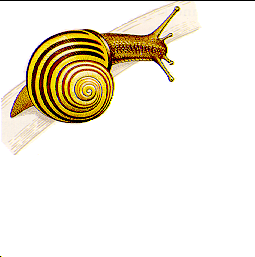
\includegraphics[height=\textheight,width=\textwidth,keepaspectratio]
    {figures/snail.png}
    \caption{The Bitmap picture of a snail.}\label{fig:snail}
\end{figure}

\begin{figure}
    \centering
    
\includegraphics[height=\textheight,width=\textwidth,keepaspectratio]
    {figures/snail_cbc.png}
    \caption{The CBC-mode encrypted picture of a snail.}\label{fig:snail_cbc}
\end{figure}

\begin{figure}
    \centering
    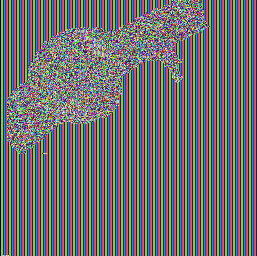
\includegraphics[height=\textheight,width=\textwidth,keepaspectratio]
    {figures/snail_ecb.png}
    \caption{The ECB-mode encrypted picture of a snail.}\label{fig:snail_ecb}
\end{figure}